
\chapter{想经济学家一样思考}

每个研究领域都有自己的语言和思考方式。
我们学习经济主要是学习其语言和思考方式。
正如你不可能在一夜之间成为一个数学家、心理学家或律师一样,
学会想经济学家一样思考也需要一些时间。


\section{作为科学家的经济学家}

经济学家研究经济的方法:
\begin{enumerate}
\item 提出理论
\item 收集数据
\item 分析数据
\item 努力证明或否定他们的理论
\end{enumerate}


科学的本质是科学的方法--冷静的建立并验证有关世界如何运行的各种理论。

\subsection{科学方法:观察、理论和进一步观察}



虽然经济学家像其他科学家一样运用理论和观察,
但他们面临着一种使其工作更具挑战性的障碍:
在经济学研究中,进行实验往往是不可能的。


\subsection{假设的作用}

假设可以使复杂的世界简单化,从而使解释这个世界变的更为容易。
科学思考的艺术就是决定做出什么假设。


\subsection{经济模型}

经济学家用由徒刑和方程组成的模型来了解世界,
经济模型忽略了许多细节,
以便使我们了解真正重要的东西。

当我们用模型来研究各种经济问题时,
所有模型都建立在一些假设之上。
经济学家利用假设撇开与所研究问题无关的许多经济细节。
所有模型都是为了加深我们对现实的理解而简化了现实。


\subsection{循环流量图}

\begin{figure}[!ht]
  \centering
  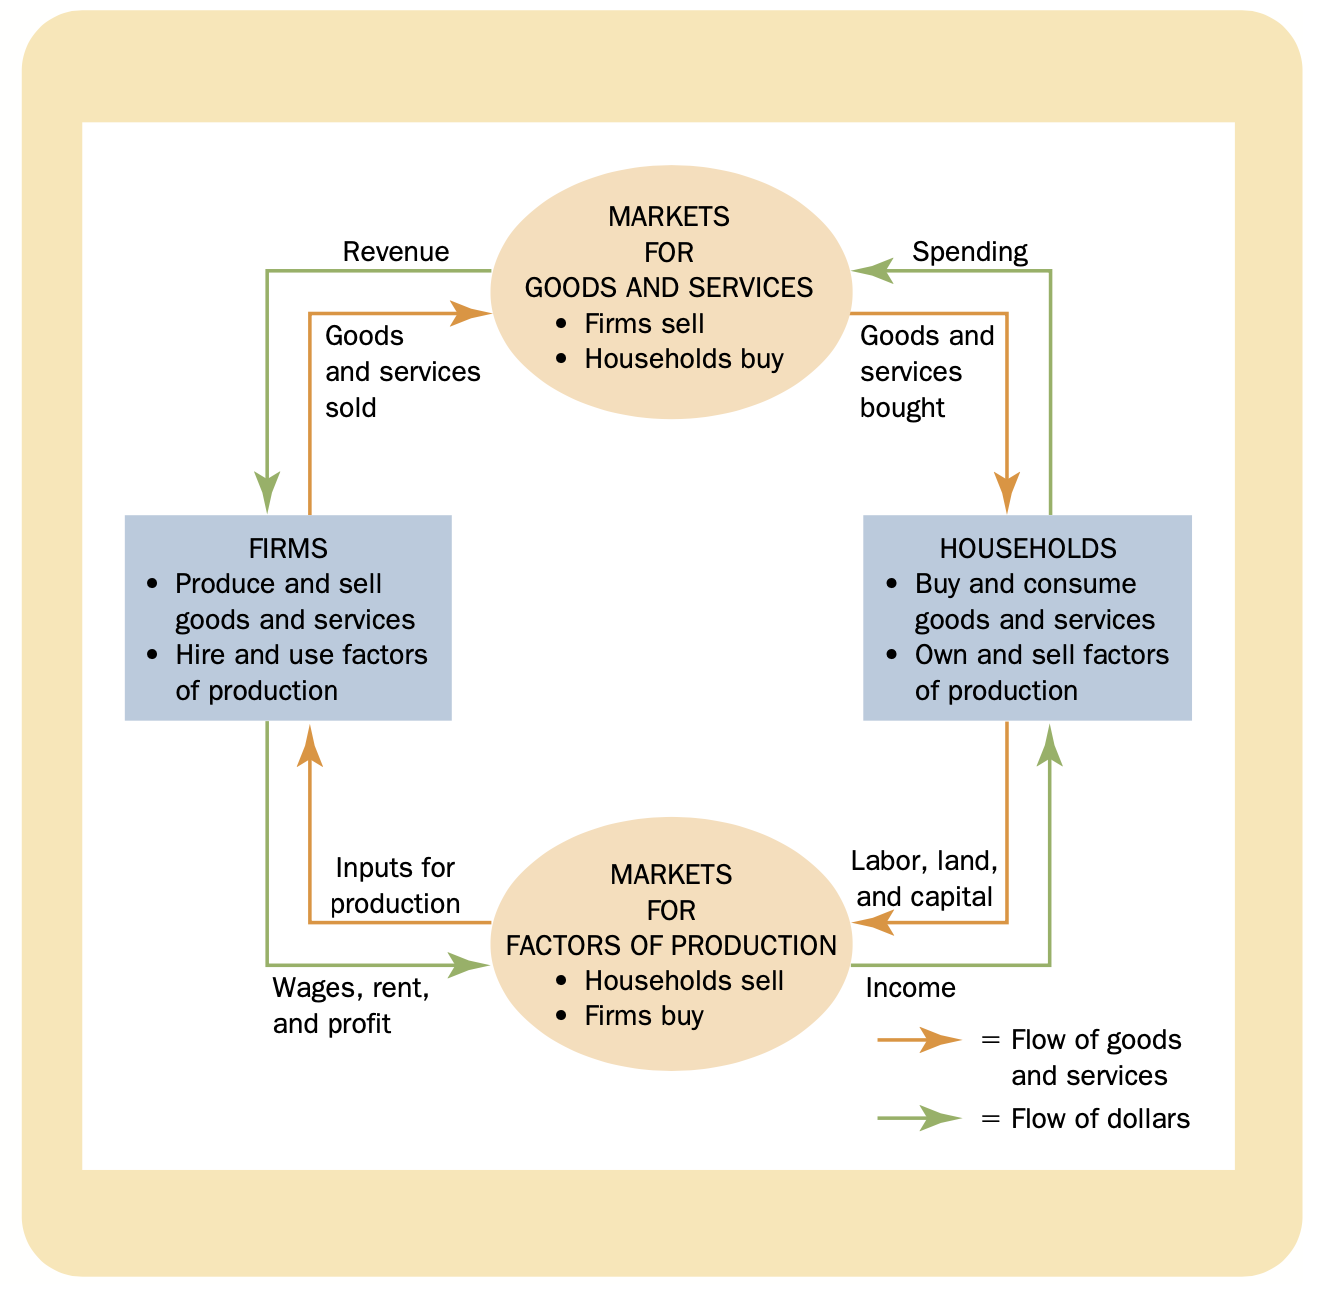
\includegraphics[width=\textwidth]{pics/circular-flow}
  \caption{循环流量图}
  \label{fig:circular-flow}
\end{figure}

在这个模型中,经济简化为只有两类决策者--企业家和家庭--组成。
企业用劳动、土地和资本(建筑物和机器)这些投入品来生产物品和服务。
这些投入品被称为生产要素。
家庭则拥有生产要素并消费企业家的所有物品与服务。


家庭和企业在两类时常上相互交易。
在物品和服务市场上,家庭是买者,而企业是卖者。
在生产要素市场上,家庭是卖者,而企业家是买者。
循环流量图提供了一种把家庭与企业之间发生的所有经济交易组织在一起的简单方法。


\subsection{生产可能性边界}

\begin{figure}[!ht]
  \centering
  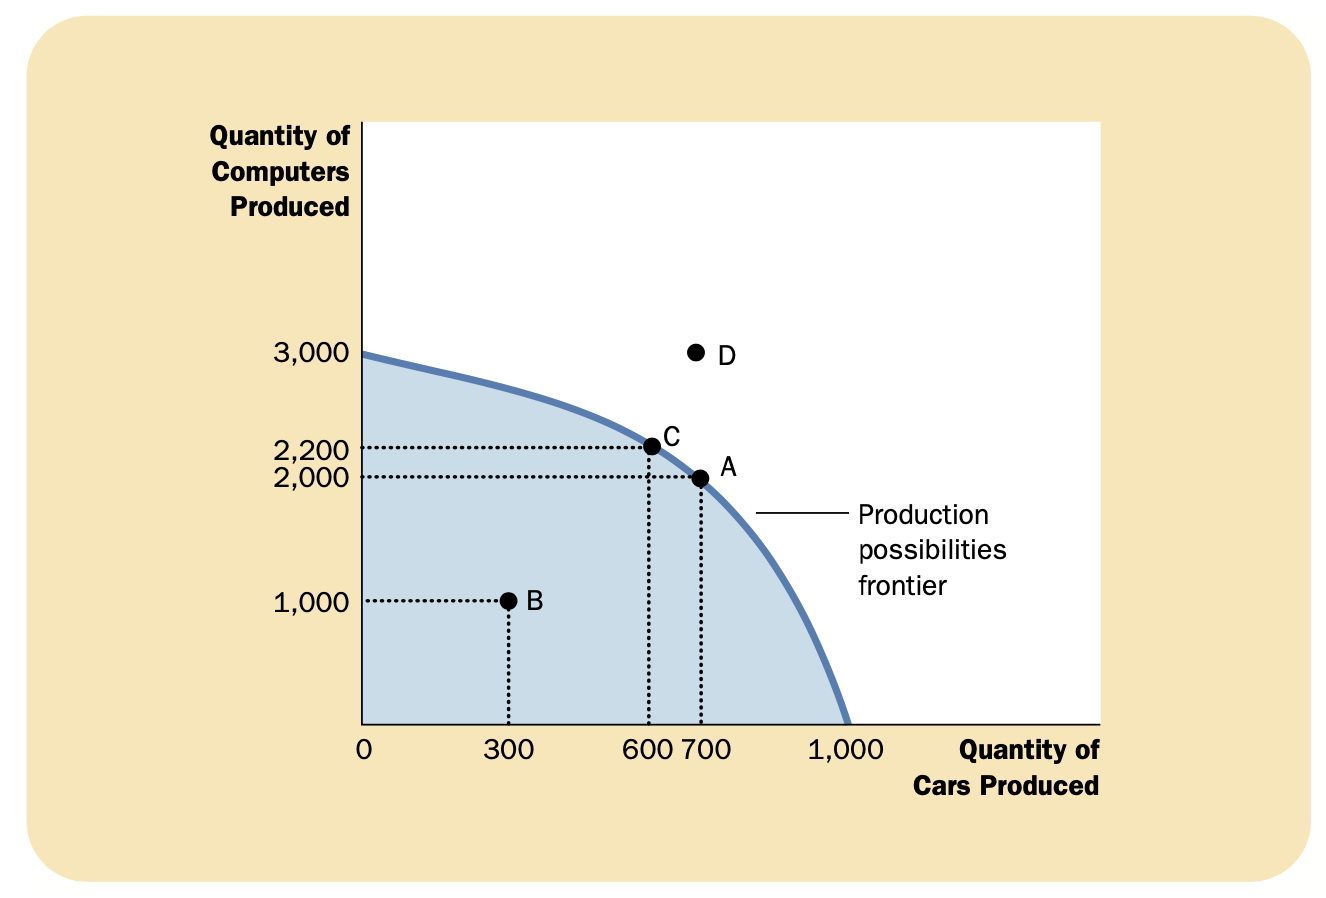
\includegraphics[width=\textwidth]{pics/the-production-possibilities-frontier}
  \caption{生产可能性边界}
  \label{fig:the-production-possibilities-frontier}
\end{figure}


虽然现实经济成千上万种物品和服务,但我们可以设想一个只生产两种物品--汽车和电脑--的经济。
生产可能性边界是一个图形,
它表明在生产要素和生产技术既定时,
一个经济所能生产的产品--在这个例子中是汽车和电脑--的数量的各种组合。


由于资源是稀缺的,因此并不是每一个想象的结果都是可行等等。
例如无法生产出D点所表示的汽车和电脑量。


如果一个经济从它可以获得的稀缺资源中获得它得到的全部东西,
就称这种结果是\emph{有效率}的。
生产可能性边界上(而不是这条线之内)的点代表了有效率的生产水平。

生产可能性边界表明在某一特定时期内生产不同物品之间的权衡取舍,
但随着时间的推移,
这种权衡取舍可以改变。

\begin{figure}[!ht]
  \centering
  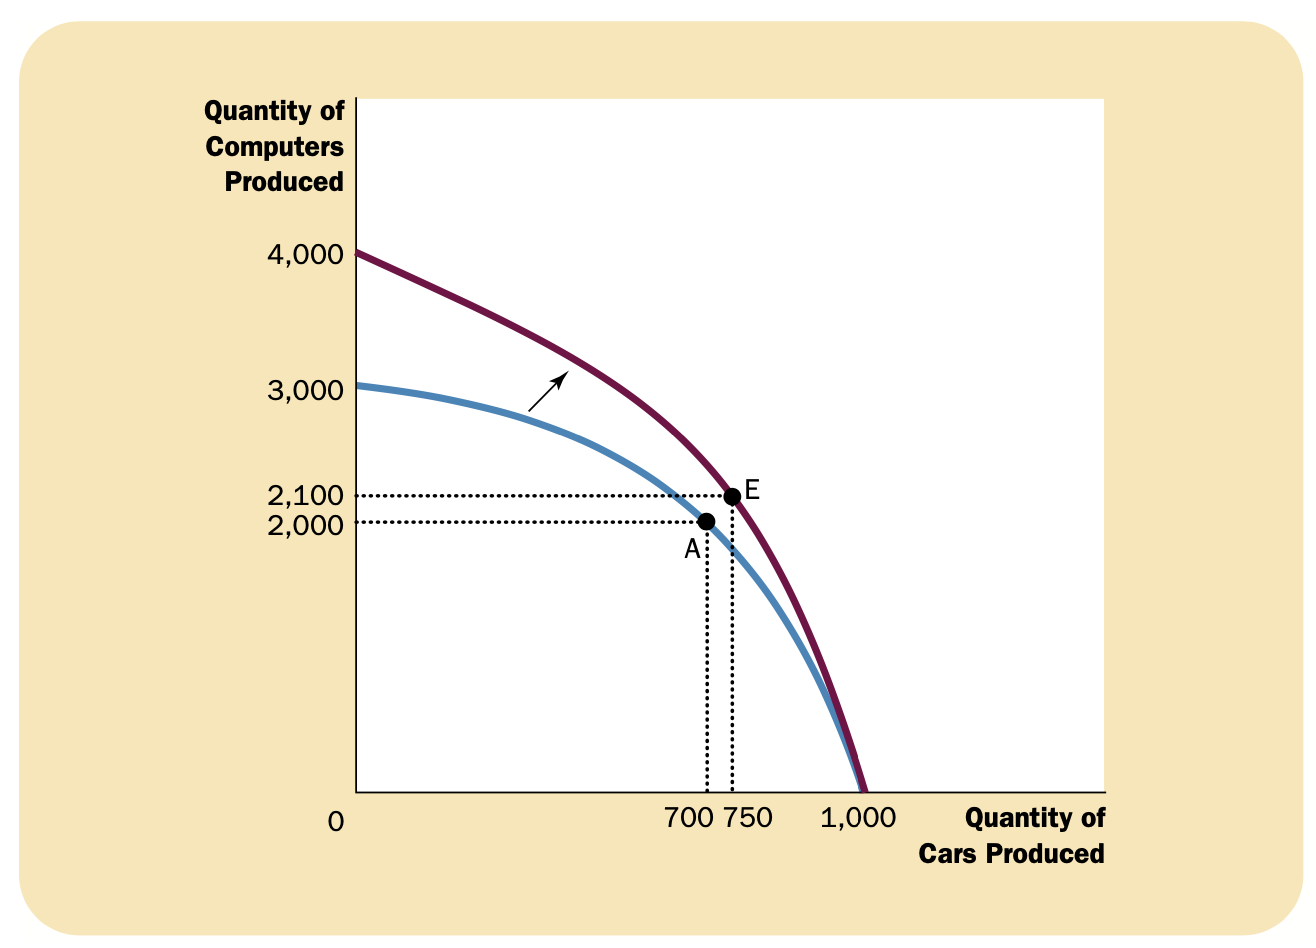
\includegraphics[width=\textwidth]{pics/a-shift-in-the-production-possibilities-frontier}
  \caption{生产可能性边界的移动}
  \label{fig:a-shift-in-the-production-possibilities-frontier}
\end{figure}


图\ref{fig:a-shift-in-the-production-possibilities-frontier}说明当经济增长时会发生的情况(例如生产电脑的技术水平的提高)。



生产可能性边界简化了复杂的经济,
以便强调一些基本但极为重要的思想:
稀缺性,效率,权衡取舍,机会成本和机会增长。




\subsection{微观经济学和宏观经济学}

经济学家在各种不同的层次上进行研究。
传统上,经济学被划分为两个大的分领域。
微观经济学研究家庭和企业如何做出决策,
以及他们如何在特定市场上相互交易。
宏观经济学研究整体经济现象。


\section{作为政策顾问的经济学家}

当经济学家试图去解释世界时,他们时科学家;
当经济学家试图去改善世界时,他们时政策顾问。



\subsection{实证分析与规范分析}

由于科学家和政策顾问有不同的目标,
所以他们也以不同的方式使用语言。


例如,假设两个人在讨论最低工资法。
\begin{verbatim}
张三:最低工资法引起失业。
李四:政府应该提高最低工资。
\end{verbatim}

张三和李四想做的事情时不同的。
张三的说法像一个科学家,他做出了一种关于世界如何运行的表述。
李四的说法像一个政策顾问,他做出了他想如何改变世界的表述。


一般来说,关于世界的表述有两种类型。
第一种类型的表述是实证的。
实证表述是描述性的,它们做出关于世界\emph{是}什么样子的表述。
第二种类型的表述是规范性的。
规范表述是规定性的,它做出关于世界\emph{应该是}什么样子的表述。


经济学的许多内容是实证的:它仅仅在努力解释世界如何运作。
但那些运行经济学的经济学家们通常有规范的目的:他们想知道如何改善经济。


\begin{verbatim}
   经济学家和政治哲学家的思想,无论正确与否,实际上都要比一般
所想象的更有力量。事实上,这个世界就是由他们统治的。那些自认为
能够免于受经济学家影响的实干家往往是某些已故经济学家的俘虏。那
些当权狂人信奉的其实也不过是若干年前某些末流文人狂妄思想的零碎
而已。                    ---- John Maynard Keynes
\end{verbatim}


\section{经济学家意见分歧的原因}

“如果让所有的经济学家围坐在一起,他们不会达成任何一个共识。”
George Bernard Shaw对经济学家的嘲讽从这句话中可见一斑。


为什么经济学家往往给决策者提供相互矛盾的建议呢?
这里有两个基本原因:
\begin{itemize}
\item 经济学家可能对世界如何运行的不同实证理论的正确性看法不一致。
\item 经济学家可能有不同的价值观,因此对政策应该努力实现的目标有不同的规范观点。
\end{itemize}


\subsection{感觉与现实}


由于科学判断的差别和价值观的不同,
经济学家之间有一些分歧是不可避免的,
但不应该夸大这种分歧。
经济学家之间的共识程度远远超出了人们有时认为的那样。


\begin{verbatim}
对专业的经济学家来说,网络游戏可能是下一个前沿。
\end{verbatim}
网游里的数据相当丰富。
而且,在网游中进行全面经济实验要容易的多。



\begin{verbatim}
经济学研究似乎并不需要任何极高的特殊天赋。与更高深的哲学或
纯科学相比,经济学难道不是...一门及其容易的学科吗?它是一门
容易的学科,但这个学科中很少有人能出类拔萃!对这个悖论的解释
也许在与杰出的经济学家应该具有罕见的各种天赋的组合。在某种
程度上,他们应该是数学家、历史学家、政治家和哲学家。他必须
了解符号符号并用文字将其表达出来。他必须根据一般性来深入思考
特殊性,并在思绪奔放的同时触及抽象与具体。他必须根据过去、
着眼现在而研究未来。他必须考虑到人性和人的制度的每一部分。
他必须同时保持坚定而客观的情绪,要像艺术家一样超然而不流俗,
但有时又要像政治家一样脚踏实地。
\end{verbatim}


\subsection{原因与结果}

当你看到一幅图被用于支持一种关于原因和结果的观点时,
应当问一下,
有没有一种被忽略的变量的变动能解释你观察到的结果,
这一点时很重要的。


